% !TEX program = pdflatex
% !BIB program = bibtex
\documentclass{article}

\usepackage{geometry}
\geometry{
a4paper,
total={170mm,257mm},
left=20mm,
top=20mm,
}
\usepackage{indentfirst}
\setlength{\parindent}{2em}
\usepackage{hyperref}
\usepackage{graphicx}
\usepackage{url}
\usepackage{multirow}
\usepackage{multicol}
\usepackage{caption}
\usepackage{float}
\usepackage{amsmath}
\usepackage{amsfonts}
\usepackage{chngcntr}
\counterwithin*{subsection}{section}
\renewcommand{\thesubsection}{\thesection.\alph{subsection}}

\usepackage{amsmath}
\DeclareMathOperator{\Tr}{Tr}

\newtheorem{theorem}{Theorem}[section]

\title{Project: Quantum Harmonic Oscillator}
\author{Dacheng Xu}
\date{2022.12.10}

\begin{document}
\maketitle
\newpage
\thispagestyle{empty}
\begin{large}
\tableofcontents
\listoffigures
\end{large}
\newpage
\setcounter{page}{1}

\begin{abstract}
    This note presents and simulates the low temperature limit calculation of quantum harmonic oscillator. By performing Wick rotation, the project derived the density matrix of the harmonic oscillator with Feynman path integral. By Monte Carlo simulation with Metropolis algorithm, the project calculates the distribution of the energy of the ground state. The theoretical prediction and simulation are aligned well. 
\end{abstract}

\textit{Keywords}: Harmonic oscillator, Monte Carlo simulation

\newpage
\thispagestyle{empty}
% \section*{Introduction}

Consider a Hamiltonian for the 1-dimensional quantum harmonic oscillator with frequency $\omega$ and mass $m$

\begin{equation}
    \hat{H} = \frac{\hat{p}^2}{2m} + \frac{m\omega^2\hat{x}^2}{2}.
\end{equation}

It is well-known that its spectrum $\hat{H}|\psi_n\rangle=E_n|\psi_n\rangle$ is given by

\begin{equation}
    E_n = \hbar\omega\left(n+\frac{1}{2}\right),
\end{equation}

and the wavefunctions are

\begin{equation}
    \langle x|\psi_n \rangle = \frac{1}{\sqrt{2^n n!}}\left(\frac{m\omega}{\pi\hbar}\right)^{1/4}e^{-\xi^2/2}H_n(\xi),
\end{equation}

where $\xi=\sqrt{m\omega/\hbar}x$ denotes dimensionless length, and $H_n(\xi)$ are Hermite polynomials:

\begin{equation}
    H_0(\xi) = 1,\ H_1(\xi) = \xi,\ H_2(\xi) = \xi^2-1,\cdots
\end{equation}

\section*{A}

The sum required to calculate the density matrix of the canonical ensemble $\hat{\rho}\sim e^{-\beta\hat{H}}$ in the position space takes the form

\begin{equation}
    \langle x'|e^{-\beta\hat{H}}|x\rangle = \sum_{m,n}\langle x'|\psi_m\rangle\langle\psi_m|e^{-\beta\hat{H}}|\psi_n\rangle\langle\psi_n|x\rangle=\sqrt{\frac{m\omega}{\pi\hbar}}\sum_n\frac{1}{2^nn!}e^{-(\xi^2+\xi'^2)/2}e^{-\beta E_n}H_n(\xi)H_n(\xi')
\end{equation}

after further evaluation,

\begin{equation}
    \langle x'|e^{-\beta\hat{H}}|x\rangle = \left(\frac{m\omega}{2\pi\hbar\sinh(\beta\hbar\omega)}\right)^{1/2} \exp\left[\frac{m\omega}{4\hbar}(x+x')^2\tanh(\frac{\beta\hbar\omega}{2})+(x-x')^2\coth(\frac{\beta\hbar\omega}{2})\right]
\end{equation}

to derive the partition function, 

\begin{equation}
    Z = \Tr e^{-\beta\hat{H}} = \int_{-\infty}^{\infty}\langle x'|e^{-\beta\hat{H}}|x\rangle\mathrm{d}x = \left(\frac{m\omega}{2\pi\hbar\sinh(\beta\hbar\omega)}\right)^{1/2} \int_{-\infty}^{\infty} \exp\left[\frac{m\omega x^2}{\hbar}\tanh(\frac{\beta\hbar\omega}{2})\right]\mathrm{d}x = \frac{e^{-\beta\hbar\omega/2}}{1-e^{-\beta\hbar\omega}}
\end{equation}

then the matrix element $\hat{\rho}$ is

when $\beta\rightarrow\infty$,

\begin{equation}
    \lim_{\beta\rightarrow\infty}\langle x'|e^{-\beta\hat{H}}|x\rangle = 0
\end{equation}

\begin{equation}
    \lim_{\beta\rightarrow\infty}Z = 0
\end{equation}

\begin{equation}
    \lim_{\beta\rightarrow\infty}\hat{\rho} = \frac{\langle x'|e^{-\beta\hat{H}}|x\rangle}{\Tr\left(\langle x'|e^{-\beta\hat{H}}|x\rangle\right)} = \sqrt{\frac{m\omega}{\pi\hbar}}\exp(-\frac{m\omega(x^2+x'^2)}{2\hbar})
\end{equation}

\begin{equation}
    \langle \hat{x}^2\rangle = \Tr\left(\hat{\rho}\hat{x}^2\right) = \int_{-\infty}^{\infty}\langle x'|x^2e^{-\beta\hat{H}}|x\rangle\mathrm{d}x = \left(\frac{m\omega}{2\pi\hbar\sinh(\beta\hbar\omega)}\right)^{1/2} \int_{-\infty}^{\infty} x^2\exp\left[\frac{m\omega x^2}{\hbar}\tanh(\frac{\beta\hbar\omega}{2})\right]\mathrm{d}x = \sqrt{\frac{\hbar}{2m\omega\tanh(\beta\hbar\omega/2)}}
\end{equation}

% \section*{b}

Now recall that the quantum-mechanical transition amplitude between two states with positions $x$ and $x'$ is in direct correspondence with the matrix element of $e^{-\beta\hat{H}}$

\begin{equation}
    \langle x',t'|x,t\rangle = \langle x'|e^{-\frac{i}{\hbar}\hat{H}(t'-t)}|x\rangle \rightarrow \langle x'|e^{-\beta\hat{H}}|x\rangle
\end{equation}

upon the substitution $(t'-t)\rightarrow -i\hbar\beta$. On the other hand, we know that the amplitude $\langle x',t'|x,t\rangle$ can be expressed as a Feynman path integral

\begin{equation}
    \langle x'=x_N,t'=t_N|x=x_0,t=t_0\rangle = \int_{x(t)=x}^{x(t')=x'}\mathcal{D}x e^{\frac{i}{\hbar}S[x(t)]} \label{eq:1}, 
\end{equation}

where we assume the timeline $t_N-t_0$ to be broken down into $N$ equal and small time intervals $\Delta t$,

\begin{equation}
    \int\mathcal{D}x \equiv \Pi_{n=1}^{N-1}\left[\int_{-\infty}^\infty\mathrm{d}x_n\sqrt{\frac{m}{2\pi i\hbar\Delta t}}\right],
\end{equation}

and $S$ is the action for our harmonic oscillator evaluated on a trajectory $x(t)$

\begin{equation}
    S[x(t)] = \int_{t_0}^{t_N}\left(\frac{1}{2}m\dot{x}^2-\frac{1}{2}m\omega^2x^2\right)\mathrm{d}s.
\end{equation}

Set classical action as $S_{\mathrm{cl}}(t,t',x,x') \equiv S[x_{\mathrm{cl}}(t)]$, then evaluate trajectory $x_{\mathrm{cl}}(s)$,

\begin{align}
    x_{\mathrm{cl}}(s) = x'\frac{\sin(\omega (s-t))}{\sin(\omega (t'-t))} + x\frac{\sin(\omega (t'-s))}{\sin(\omega (t'-t))} \\
    \frac{\mathrm{d}x_{\mathrm{cl}}}{\mathrm{d}s} = \omega\left(x'\frac{\cos(\omega (s-t))}{\sin(\omega (t'-t))} - x\frac{\cos(\omega (t'-s))}{\sin(\omega (t'-t))}\right)
\end{align}

\subsection*{b.i}

Then $S[x_{\mathrm{cl}}(s)]$ is

\begin{equation}
    S[x_{\mathrm{cl}}(t)] = \int_{t}^{t'}\left(\frac{1}{2}m\dot{x}^2-\frac{1}{2}m\omega^2x^2\right)\mathrm{d}s = \frac{m\omega}{2\sin(\omega(t'-t))}\left[(x^2+x'^2)\cos(\omega(t'-t))-2x'x\right]
\end{equation}

Decomposition of the trajectory $x(t) = x_{\mathrm{cl}}(t)+y(t)$ into the classical part $x_{\mathrm{cl}}(t)$ and the fluctuation $y(t)$ around it allows to evaluate the path integral (\ref{eq:1}) up to a normalization constant

\begin{equation}
    \langle x'=x_N,t'=t_N|x=x_0,t=t_0\rangle = e^{\frac{i}{\hbar}S_{\mathrm{cl}}(t,t',x,x')}\int_{y(t)=0}^{y(t')=0}\mathcal{D}y e^{\frac{i}{\hbar}\int_t^{t'}\left(\frac{1}{2}m\dot{y}^2-\frac{1}{2}m\omega^2y^2\right)}.
\end{equation}

Since the integral over $y$ does not depend on $x$ or $x'$, we can limit ourselves to

\begin{equation}
    \langle x'=x_N,t'=t_N|x=x_0,t=t_0\rangle \sim e^{\frac{i}{\hbar}S_{\mathrm{cl}}(t,t',x,x')} \label{eq:2},
\end{equation}

with the normalization factor that we can evaluate later.

\subsection*{b.ii}

By performing the Wick rotation $(t'-t)\rightarrow -i\hbar\beta$ of (\ref{eq:2}),

\begin{equation}
    \langle x'|e^{-\beta\hat{H}}|x\rangle = \exp\left[-\frac{m\omega}{2\hbar\sinh(\beta\hbar\omega)}\left((x^2+x'^2)\cosh(\beta\hbar\omega)-2x'x\right)\right]
\end{equation}

\begin{equation}
    Z = \Tr\left(e^{-\beta\hat{H}}\right) = \int_{-\infty}^{\infty}\langle x'|e^{-\beta\hat{H}}|x\rangle\mathrm{d}x \sim \sqrt{\frac{\pi\hbar}{m\omega}\coth(\frac{\beta\hbar\omega}{2})}.
\end{equation}

Full expression for the density matrix of the harmonic oscillator is

\begin{equation}
    \hat{\rho} \sim \sqrt{\frac{m\omega}{\pi\hbar}\tanh(\frac{\beta\hbar\omega}{2})} \exp\left(-\frac{m\omega}{2\hbar\sinh(\beta\hbar\omega)}\left[(x^2+x'^2)\cosh(\beta\hbar\omega)-2x'x\right]\right).
\end{equation}

When $\beta\rightarrow\infty$,

\begin{equation}
    \lim_{\beta\rightarrow\infty}\hat{\rho} = \sqrt{\frac{m\omega}{\pi\hbar}}\exp(-\frac{m\omega(x^2+x'^2)}{2\hbar})
\end{equation}

The expression of $\hat{\rho}$ at low temperature limit is aligned with previous section.

But actually the precise expression of $\langle x'=x_N,t'=t_N|x=x_0,t=t_0\rangle$ is

\begin{equation}
    \langle x'=x_N,t'=t_N|x=x_0,t=t_0\rangle = \sqrt{\frac{m\omega}{2i\pi\hbar\sin(\omega(t'-t))}}\exp\left(\frac{im\omega}{2\hbar\sin(\omega(t'-t))}\left[(x'^2+x^2)\cos(\omega(t'-t))\right]-2x'x\right)
\end{equation}

% \section*{c}

By using the rotation to imaginary time aka inverse temperature, it becomes possible to deal with the path integral (\ref{eq:1}) numerically. Suppose $\hbar=k_b=m=\omega=1$. Upon Wick rotation $\Delta t\rightarrow -ia,t\rightarrow-i\tau$, our path integral takes the form

\begin{equation}
    \langle x'=x_N,t'=t_N|x=x_0,t=t_0\rangle = \int_{x(\tau)=x}^{x(\tau')=x'}\mathcal{D}x\exp\left[-\sum_{i=1}^{N}a\left(\frac{(x_{i}-x_{i-1})^2}{2a^2}+\frac{x_i^2}{2}\right)\right]
\end{equation}

In order not to deal with the boundary conditions, we can trace over them, obtaining an analog of the partition function $Z$, which can then be used to calculate the expectation values of different operators. In particular, we will be interested in the energy of the ground state of the harmonic oscillator that, by a virial theorem, is simply given by the $\langle\hat{x}^2\rangle$. In terms of the path integral, we have

\begin{equation}
    \langle\hat{x}^2\rangle = \frac{(\Pi_{i=0}^{N-1}\int \mathrm{d}x_i)x_j^2\exp\left[-\sum_{i=1}^{N}a\left(\frac{(x_{i}-x_{i-1})^2}{2a^2}+\frac{x_i^2}{2}\right)\right]}{(\Pi_{i=0}^{N-1}\int \mathrm{d}x_i)\exp\left[-\sum_{i=1}^{N}a\left(\frac{(x_{i}-x_{i-1})^2}{2a^2}+\frac{x_i^2}{2}\right)\right]}
\end{equation}

We can simulate the $x_j$ by sampling from N-dimensional space, with Metropolis algorithm. 

\begin{figure}
    \centering
    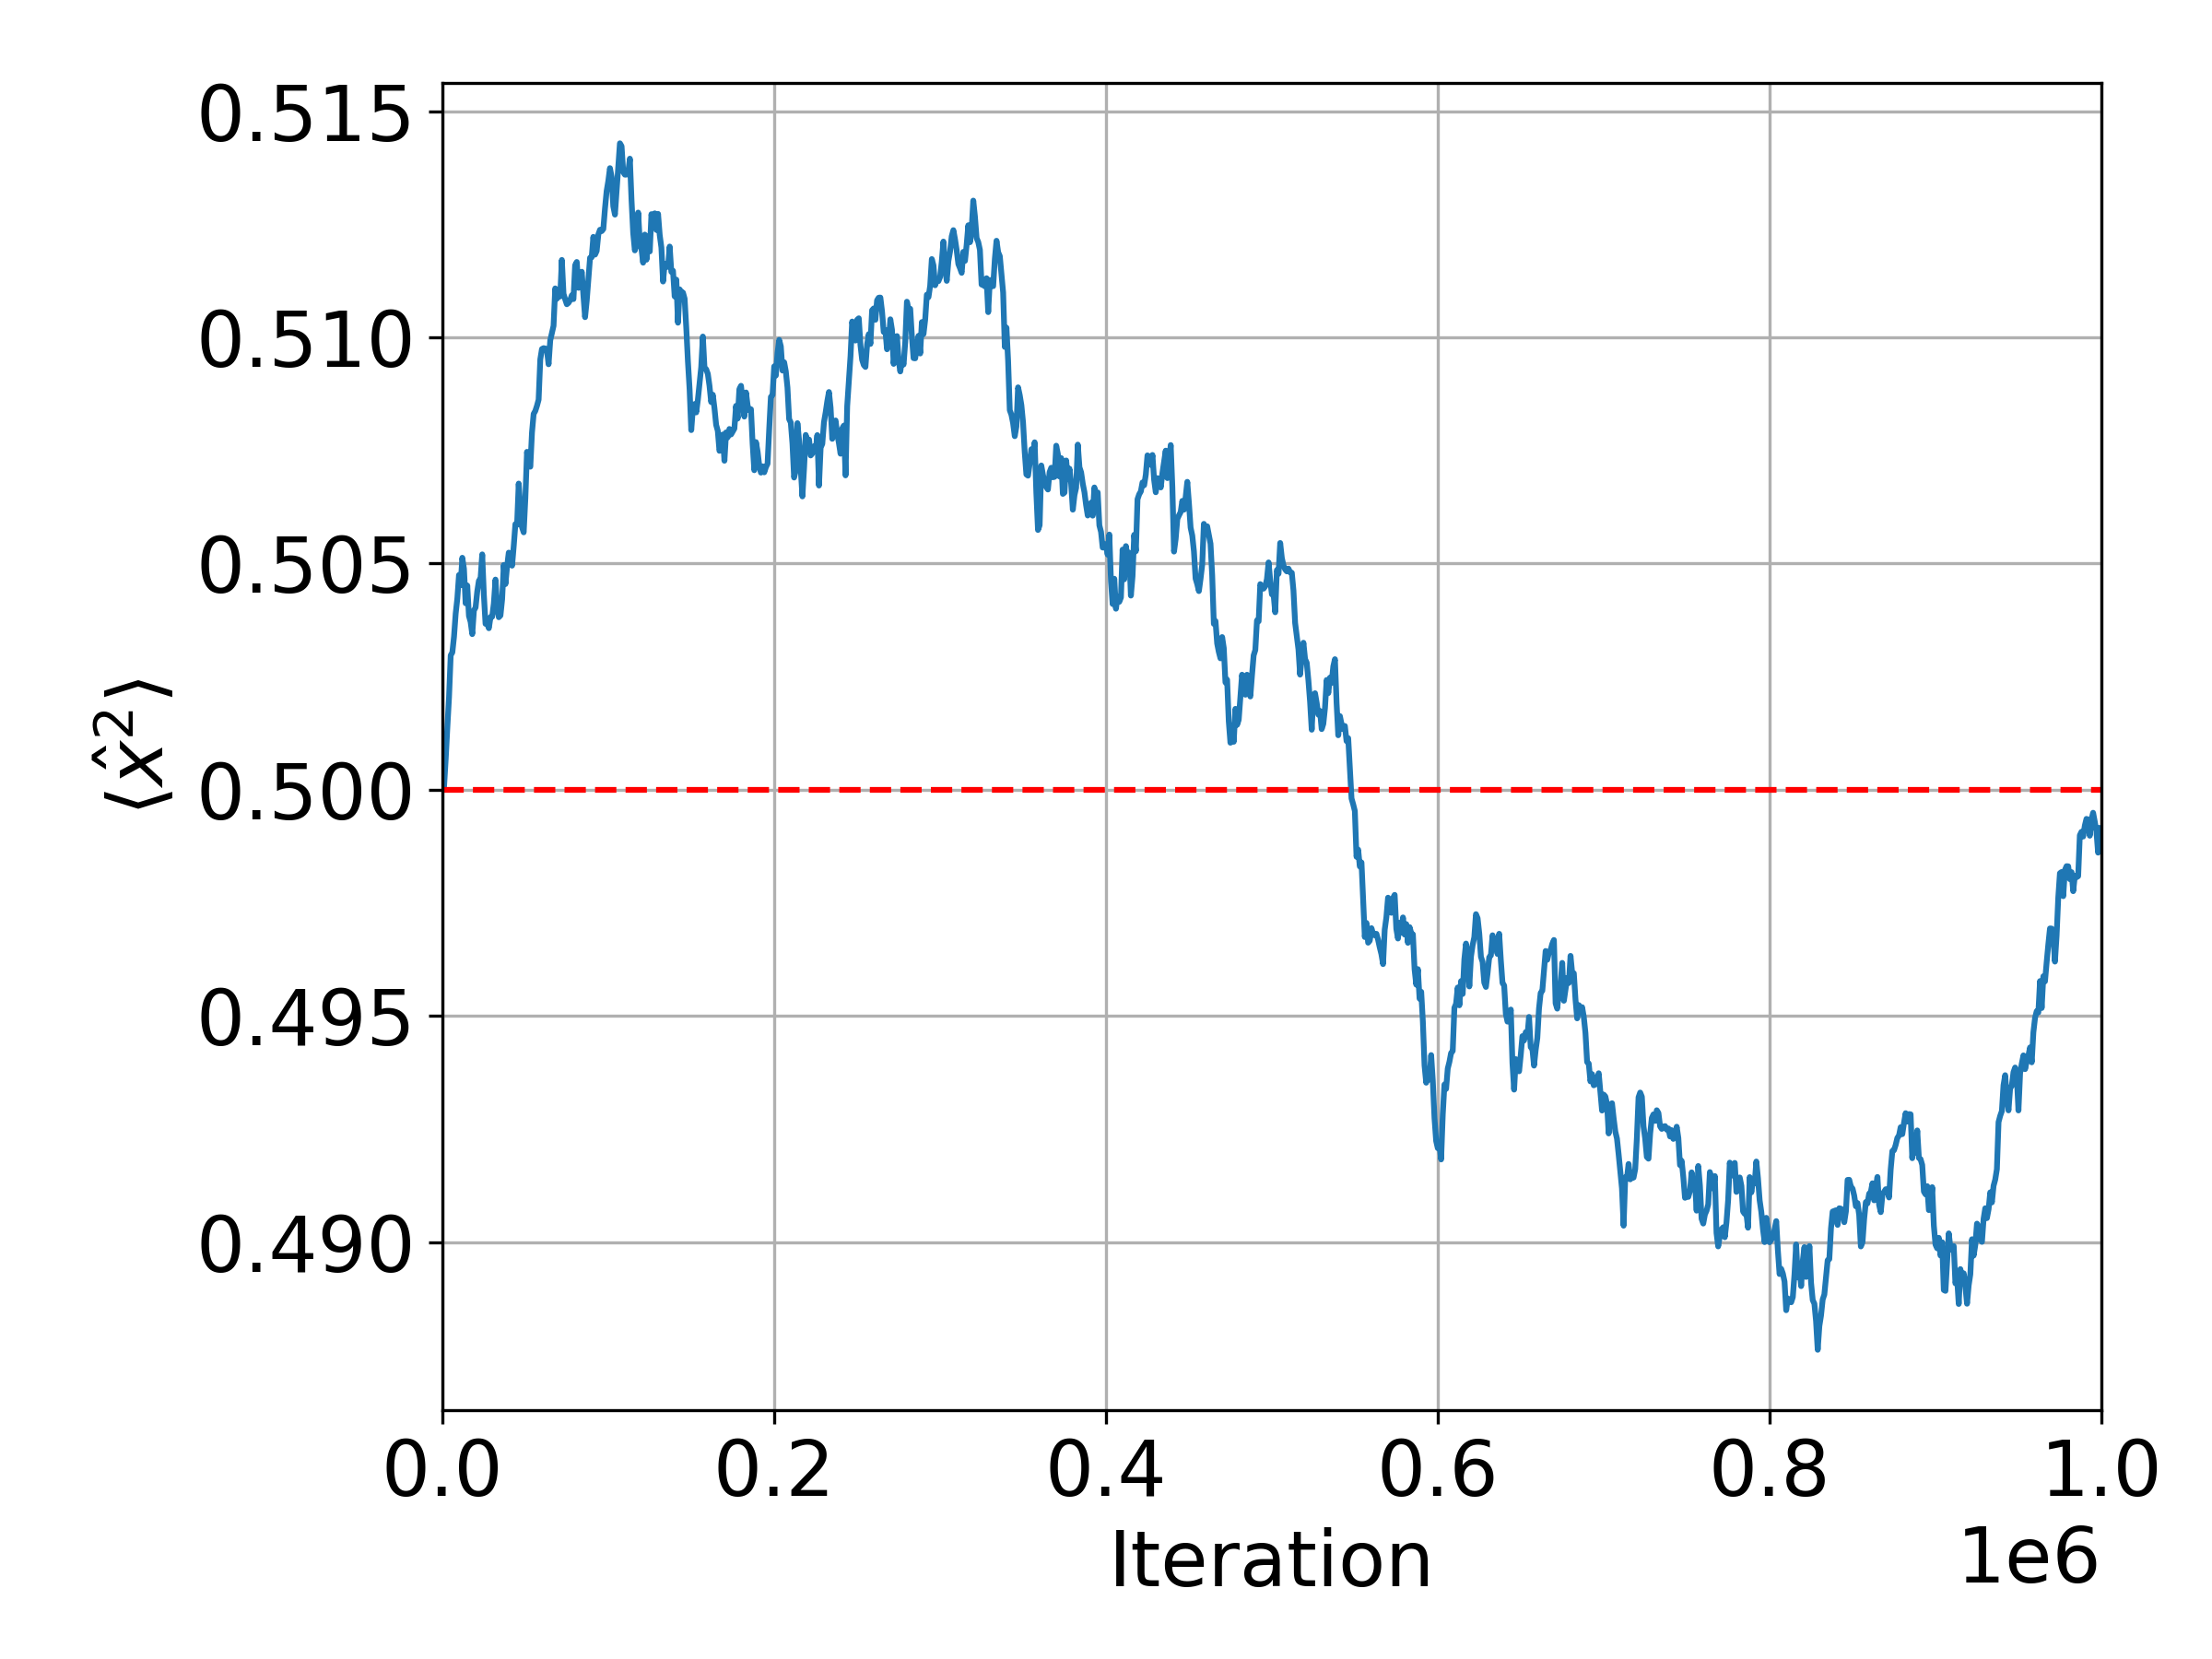
\includegraphics[width=0.6\linewidth]{figures/iterations.png}
    \caption{$\langle\hat{x}^2\rangle$ of N $x_j^2$ as function of iteration(the number of sweeps) through Metropolis algorithm\label{fig:1}}
\end{figure}

The predicted value of $\langle\hat{x}^2\rangle$ in low temperature limit from (\ref{eq:3}) is $0.5$, while the figure below shows the simulated $\langle\hat{x}^2\rangle$.

\begin{figure}
    \centering
    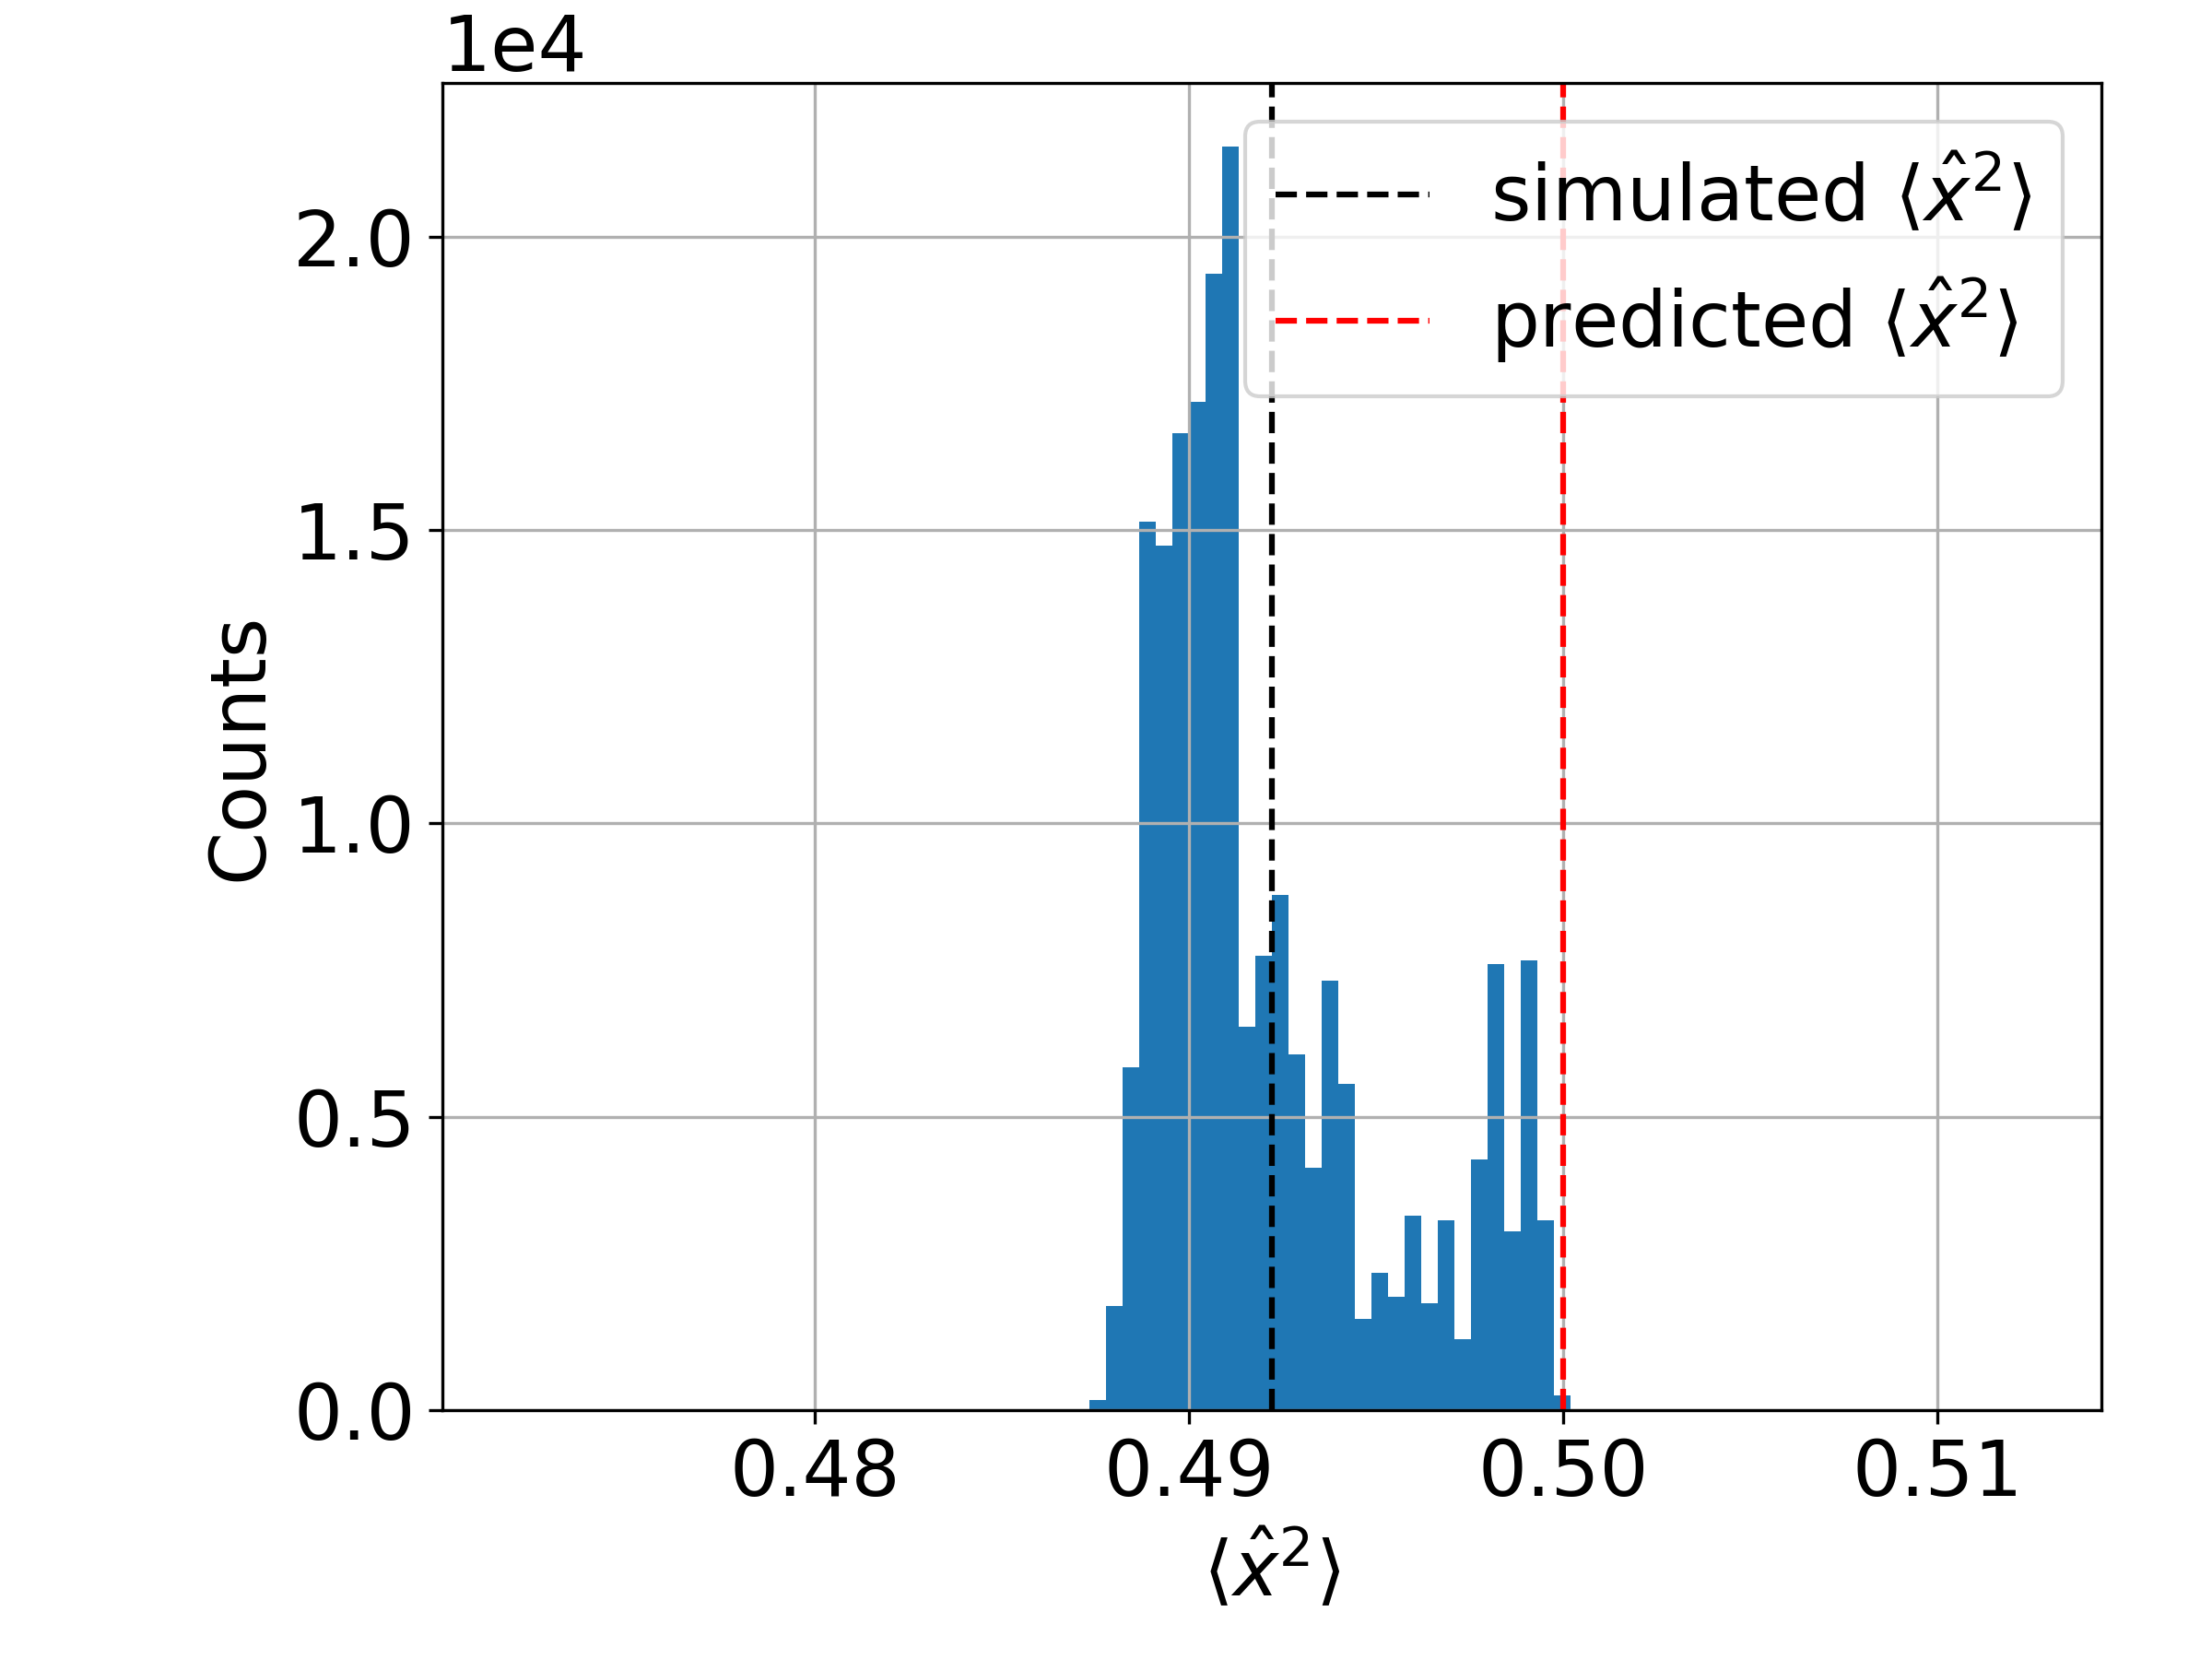
\includegraphics[width=0.6\linewidth]{figures/x2_hist.png}
    \caption{Comparison between simulated and predicted $\langle\hat{x}^2\rangle$}
\end{figure}

The difference between simulated and predicted $\langle\hat{x}^2\rangle$ is mainly due to statistical fluctuation and lack of number of sweeps. As we can see large fluctuation in Fig. \ref{fig:1}, more iteration is necessary. 

The code of these simulation is uploaded to a python notebook in GitHub\footnote{The source codes are available on GitHub \url{https://github.com/dachengx/QuantumHO/blob/main/simulation.ipynb}.}.


% \nocite{*}
\bibliographystyle{unsrt}
\bibliography{ref}
\newpage
% \section*{Appendix: Python code}
\begin{lstlisting}
a = 1e-2

# number of simulation
M = 1000000

# number of runner
N = 1000

def logpdf(array, a=1):
    # return -a * np.sum(((array[0] - array[1]) ** 2) / (2 * a ** 2) + array[0] ** 2 / 2)
    _array = np.diff(np.append(array, array[0]))
    return -a * np.sum(np.power(_array, 2) / (2 * a ** 2) + np.power(array, 2) ** 2 / 2)

def metropolis(array, i, a):
    _array = array.copy()
    _array[i] += np.random.normal(scale=a)

    # delta = logpdf(np.array([_array[i], _array[(i-1+N)//N]]), a=a)
    # delta -= logpdf(np.array([array[i], array[(i-1+N)//N]]), a=a)
    delta = logpdf(_array, a=a) - logpdf(array, a=a)
    r = np.random.uniform()
    if delta > np.log(r):
        return _array
    else:
        return array

def x2_mean(a):
    # return 1 / (2 * np.tanh(a * N / 2))
    return 1 / 2

# Metropolis algorithm
for i, j in tqdm(zip(range(1, M), indices[1:]), total=M-1, miniters=100):
    array_repo[i] = metropolis(array_repo[i-1], j, a)

\end{lstlisting}


\end{document}
